% ==============================================================================
% Monografia - Áurea Santos de Oliveira
% Capítulo 4 - Indexação do CDC com o GraphRAG
% ==============================================================================
\chapter{Indexação do Código de Defesa do Consumidor}
\label{sec-indexacao}

Este capítulo descreve como o GraphRAG foi aplicado ao CDC: da obtenção e estruturação do texto da lei à análise do grafo de conhecimento gerado. A Seção~\ref{sec-indexacao-inicial} apresenta a primeira versão do projeto, executada com modelos locais, e os motivos da mudança para modelos em nuvem. As seções~\ref{sec-indexacao-corpus} e~\ref{sec-indexacao-segmentacao} tratam da preparação do corpus. As seções~\ref{sec-indexacao-modelos} a~\ref{sec-indexacao-prompts} descrevem as decisões de configuração: modelos, temperatura, taxonomia e \textit{prompts}. As seções~\ref{sec-indexacao-execucao} a~\ref{sec-indexacao-release} apresentam a execução da indexação, o grafo resultante, o custo e a publicação do índice.

%%% Início de seção. %%%
\section{Primeira Versão: Modelos Locais}
\label{sec-indexacao-inicial}

A primeira versão da prova de conceito foi executada inteiramente na máquina da autora, com o objetivo de evitar custos de API. Os modelos eram servidos pelo Ollama \cite{ollama} em um contêiner: o \code{llama3.1:8b}, com janela de contexto ampliada para 8.192 \textit{tokens}, para geração, e o \code{nomic-embed-text} para \textit{embeddings}. Como a máquina não dispõe de GPU, a configuração limitava o GraphRAG a uma requisição simultânea, com tempo máximo de 30 minutos por chamada.

Essa versão permitiu montar o ambiente em contêineres, entender o \textit{pipeline} e construir o primeiro visualizador do grafo, mas mostrou-se inviável para o trabalho por três motivos. Primeiro, o tempo: cada chamada ao modelo levava em torno de sete minutos, e a indexação completa, horas. Segundo, a qualidade: o modelo pequeno produzia extrações incompletas e inconsistentes, com tipos de entidade e nomes fora do padrão. Terceiro, a configuração: os \textit{prompts}, gerados pelo ajuste automático com o próprio modelo local, usavam tipos de entidade em inglês descobertos pelo modelo (\textit{law}, \textit{consumer}, \textit{business}, \textit{government}, \textit{product}, \textit{service}), e não a taxonomia definida na configuração, e a pasta de entrada continha, além do texto da lei, uma versão antiga e incompleta do CDC, de modo que dois documentos sobrepostos eram indexados. A configuração local foi preservada como alternativa no repositório, idêntica à de nuvem exceto pelos modelos, e o trabalho seguiu com modelos em nuvem.

%%% Início de seção. %%%
\section{Preparação do Corpus}
\label{sec-indexacao-corpus}

\subsection{Fonte e estratégia}
\label{sec-indexacao-corpus-fonte}

O texto do CDC foi obtido da versão compilada publicada no portal da legislação federal \cite{brasil1990cdc}, que incorpora as alterações posteriores e mantém os dispositivos vetados e revogados com a respectiva indicação. Em vez de indexar o texto bruto -- o que deixaria a segmentação cortar artigos ao meio e perderia a hierarquia --, optou-se por estruturar o texto em \textbf{um registro por artigo}. Essa escolha segue a própria técnica legislativa, que define o artigo como unidade básica da lei (Seção~\ref{sec-referencial-juridico-estrutura}), e faz com que cada unidade de texto do GraphRAG corresponda a um artigo completo.

\subsection{O \textit{parser} da legislação}
\label{sec-indexacao-corpus-parser}

Foi desenvolvido em Python um \textit{parser} que lê o texto bruto e reconhece, por expressões regulares, os níveis da hierarquia da Lei Complementar nº 95/1998 \cite{brasil1998lc95} (parte, livro, título, capítulo, seção e subseção) e o início de cada artigo. Para cada artigo, gera um registro com a identificação da lei, o número e o nome de cada nível da hierarquia em que o artigo se encontra, a situação normativa e o texto completo (\textit{caput}, parágrafos, incisos e alíneas). O \textit{parser} foi escrito de forma genérica, para poder ser reaproveitado em outras leis federais. A Listagem~\ref{lst-registro-json} mostra um registro.

\begin{lstlisting}[caption={Registro de um artigo no arquivo \code{cdc.json} (campos nulos omitidos; texto abreviado).}, label=lst-registro-json]
{
  "id": "cdc_art_49",
  "artigo_num": "49",
  "lei_sigla": "CDC",
  "lei_nome": "Código de Defesa do Consumidor",
  "lei_numero": "Lei nº 8.078, de 11 de setembro de 1990",
  "titulo_num": "I",   "titulo_nome": "Dos Direitos do Consumidor",
  "capitulo_num": "VI", "capitulo_nome": "Da Proteção Contratual",
  "secao_num": "I",    "secao_nome": "Disposições Gerais",
  "situacao": "vigente",
  "dispositivos_vetados_ou_revogados": [],
  "text": "Art. 49. O consumidor pode desistir do contrato, no prazo de 7 dias ..."
}
\end{lstlisting}

A primeira versão do \textit{parser}, herdada da fase inicial do projeto, apresentava problemas que foram corrigidos antes da indexação (Tabela~\ref{tab-parser-problemas}). O mais grave era a perda do sufixo de letra dos artigos acrescentados por leis posteriores, que fazia os artigos 54 e 54-A a 54-G receberem o mesmo identificador. Como o GraphRAG usa o identificador do documento, registros com identificadores repetidos se confundiriam. O \textit{parser} passou a falhar caso encontre identificadores duplicados.

\begin{table}[htb]
\centering
\caption{Problemas corrigidos no \textit{parser} da legislação.}
\label{tab-parser-problemas}
\footnotesize
\begin{tabular}{L{4.4cm} L{4.4cm} L{5.4cm}}
\toprule
\textbf{Problema} & \textbf{Causa} & \textbf{Correção} \\
\midrule
Identificadores repetidos (arts. 54 e 54-A a 54-G; 42-A; 104-A a 104-C) & A expressão regular do artigo descartava o sufixo de letra & O número do artigo inclui o sufixo e o identificador inclui a sigla da lei (\code{cdc\_art\_54-A}) \\
Cabeçalhos como ``Art. 11º'' e ``Art. 54º-C'' & O cabeçalho era remontado sempre com ordinal & Regra da LC nº 95/1998: ordinal até o nono artigo, cardinal a partir do décimo \\
Capítulo VI-A lido como ``VI'', com nome ``-A'' & A regra dos níveis da hierarquia não aceitava sufixo & Níveis com sufixo de letra; nome lido da linha seguinte \\
Artigos inteiros marcados como vetados quando apenas um parágrafo o era (ex.: arts. 6º e 37) & Busca da expressão ``(Vetado)'' em todo o texto do artigo & Novos campos de situação, descritos a seguir \\
\bottomrule
\end{tabular}
\end{table}

\subsection{Dispositivos vetados e revogados}
\label{sec-indexacao-corpus-vetados}

Uma decisão importante foi \textbf{manter} no corpus todo o texto vetado ou revogado. Do ponto de vista jurídico, o registro de um veto também é informação: saber que o art. 54-E, que seria incluído pela Lei nº 14.181/2021 \cite{brasil2021lei14181}, foi vetado responde a uma pergunta legítima sobre a lei. Para que essa informação seja representada corretamente, cada registro recebe dois campos:

\begin{itemize}
    \item \code{situacao}: \code{vigente}, \code{vetado} ou \code{revogado}, referente ao artigo como um todo;
    \item \code{dispositivos\_vetados\_ou\_revogados}: os parágrafos, incisos ou alíneas vetados ou revogados dentro de um artigo vigente -- por exemplo, para o art. 51, os incisos V e XIX e o § 3º.
\end{itemize}

O CDC compilado resultou em 130 artigos, dos quais 12 inteiramente vetados (arts. 11, 15, 16, 45, 54-E, 62, 85, 86, 89, 96, 108 e 109), e 30 dispositivos vetados distribuídos em 21 artigos vigentes. O \textit{parser} oferece uma opção para gerar a versão sem os dispositivos vetados (118 artigos), o que permite, se desejado, comparar os dois cenários.

\subsection{Configuração da entrada}
\label{sec-indexacao-corpus-entrada}

O arquivo resultante (\code{cdc.json}) é lido pelo GraphRAG no formato JSON, com o campo \code{id} como identificador e título do documento e o campo \code{text} como conteúdo. Os demais campos ficam disponíveis como metadados. Os nomes dos campos foram mantidos em português de propósito, já que aparecem para o modelo no início de cada trecho, como descrito a seguir.

%%% Início de seção. %%%
\section{Segmentação}
\label{sec-indexacao-segmentacao}

O tamanho das unidades de texto foi mantido no padrão de 1.200 \textit{tokens}, com sobreposição de 100. Como o maior artigo do CDC tem 781 \textit{tokens} (a média é de 182), cada artigo cabe inteiro em uma unidade de texto: o índice tem 130 unidades, uma por artigo, e nenhuma mistura artigos diferentes ou corta um artigo ao meio.

Para preservar a hierarquia da lei, foi utilizada a opção \code{prepend\_metadata}, que insere no início de cada unidade de texto a sigla da lei, os nomes do título, do capítulo e da seção e a situação do artigo (Listagem~\ref{lst-chunk}). Com isso, o modelo sabe, ao extrair entidades do art. 39, que ele está no capítulo das práticas comerciais e na seção das práticas abusivas, e sabe, ao processar o art. 54-E, que ele foi vetado. A mesma informação aparece para o modelo nas consultas, sempre que uma unidade de texto é incluída no contexto.

\begin{lstlisting}[caption={Início de uma unidade de texto, com os metadados inseridos pelo \code{prepend\_metadata}.}, label=lst-chunk]
lei_sigla: CDC.
titulo_nome: Dos Direitos do Consumidor.
capitulo_nome: Da Proteção Contratual.
secao_nome: Disposições Gerais.
situacao: vigente.
Art. 49. O consumidor pode desistir do contrato, no prazo de 7 dias a contar de sua assinatura
ou do ato de recebimento do produto ou serviço, sempre que a contratação de fornecimento de
produtos e serviços ocorrer fora do estabelecimento comercial, especialmente por telefone ou
a domicílio. ...
\end{lstlisting}

%%% Início de seção. %%%
\section{Escolha dos Modelos}
\label{sec-indexacao-modelos}

Com o corpus pequeno (cerca de 24 mil \textit{tokens} nas 130 unidades de texto), o custo da indexação é dominado pelo número de chamadas e pelo tamanho dos \textit{prompts}, e não pelo volume de texto. A estratégia adotada foi usar, em cada etapa, o modelo mais barato capaz de executá-la bem, conforme a Tabela~\ref{tab-modelos}. O GraphRAG permite essa combinação porque cada etapa referencia um modelo nomeado na configuração (Seção~\ref{sec-graphrag-config-modelos}). Foram definidos dois modelos de geração -- \code{strong\_model} (\code{gpt-6.1-sol}) e \code{cheap\_model} (\code{gpt-6-luna}) -- e um de \textit{embeddings}.

\begin{table}[htb]
\centering
\caption{Modelos utilizados em cada etapa.}
\label{tab-modelos}
\footnotesize
\begin{tabular}{L{4.6cm} L{3.4cm} L{6.2cm}}
\toprule
\textbf{Etapa} & \textbf{Modelo} & \textbf{Justificativa} \\
\midrule
Extração de entidades e relações & \code{gpt-6.1-sol} & Define a qualidade do grafo; é a etapa mais importante. \\
Resumo de descrições & \code{gpt-6-luna} & Tarefa simples: fundir descrições da mesma entidade. \\
Relatórios de comunidade & \code{gpt-6.1-sol} & Base das buscas global e DRIFT. \\
Respostas das consultas (todas as modalidades) & \code{gpt-6.1-sol} & O mesmo modelo gerador em todas as modalidades, para que a comparação dependa apenas da recuperação. \\
\textit{Embeddings} & \code{text-embedding-3-large} & Vetores de 3.072 dimensões; custo desprezível para o tamanho do corpus. \\
\bottomrule
\end{tabular}
\end{table}

A OpenAI foi escolhida como provedor principal por três razões: o GraphRAG foi desenvolvido e testado pela Microsoft com modelos dessa família, o que torna a avaliação mais fiel ao funcionamento previsto da ferramenta; um único provedor fornece tanto os modelos de geração quanto os de \textit{embeddings}, com uma única chave de API; e seus modelos de \textit{embeddings} estão entre os de menor custo. Como o GraphRAG acessa os modelos pelo LiteLLM, configurações equivalentes para outros provedores (Anthropic e Google) foram preparadas e mantidas no repositório, permitindo a troca sem alteração de código.

Antes da indexação, foi criado um \textit{script} de teste que lê os modelos configurados e faz uma chamada mínima a cada um, de duas formas: como na indexação e com os parâmetros usados pela busca DRIFT. O teste custa frações de centavo e revelou, antes de qualquer gasto relevante, duas restrições dos modelos escolhidos: eles não aceitam o parâmetro \code{max\_tokens}, apenas \code{max\_completion\_tokens} (que o GraphRAG 3 já utiliza), e só aceitam temperatura igual a 1. Revelou também que a versão do LiteLLM instalada com o GraphRAG não reconhece esses modelos e, por isso, não filtra automaticamente os parâmetros não suportados, que precisam ser definidos de forma compatível na configuração.

%%% Início de seção. %%%
\section{Temperatura}
\label{sec-indexacao-temperatura}

A restrição de temperatura motivou uma análise de como o GraphRAG trata esse parâmetro. Na versão 3, a configuração de modelos passou a usar argumentos genéricos de chamada, sem temperatura padrão; assim, a indexação e as buscas local, global e básica usam o padrão do provedor, que é 1. A busca DRIFT, porém, manteve campos próprios de temperatura com valor padrão 0 -- herança da versão 2, em que todos os modelos usavam temperatura 0 por padrão. O resultado é uma inconsistência entre modalidades, e, com modelos que só aceitam temperatura 1, a DRIFT falharia com erro de parâmetro.

A decisão foi fixar explicitamente a temperatura 1 nos argumentos de chamada dos dois modelos de geração e nos dois campos da DRIFT. Assim, todas as etapas e todas as modalidades usam a mesma temperatura, e ela deixa de ser uma variável de confusão na comparação com o \textit{baseline}. A consequência metodológica é que as respostas variam entre execuções da mesma pergunta. Por isso, a avaliação (Capítulo~\ref{sec-avaliacao}) foi planejada sobre um índice congelado, igual para todas as modalidades, e com repetições de cada pergunta, o que permite medir também a consistência das respostas. Como se verá, a temperatura não é a única fonte de variação: a busca global embaralha os relatórios antes de formar os lotes, e a DRIFT sorteia o modelo de formato da resposta hipotética e as perguntas aprofundadas.

%%% Início de seção. %%%
\section{Taxonomia de Entidades}
\label{sec-indexacao-taxonomia}

Os tipos de entidade definem a ontologia do grafo: o modelo só extrai entidades dos tipos listados. A taxonomia inicial do projeto tinha oito tipos (artigo, direito, obrigação, sanção, órgão fiscalizador, relação de consumo, fornecedor e consumidor) e apresentava problemas: faltavam conceitos centrais do CDC, como produto, serviço, contrato, práticas abusivas, crimes e ações coletivas; ``órgão fiscalizador'' não abrangia o Ministério Público, a Defensoria Pública, o Poder Judiciário e as associações; ``relação de consumo'' é um conceito, e não uma categoria de entidades; ``sanção'' misturava sanções administrativas e penais; e ``artigo'' não contemplava remissões a outras normas.

A taxonomia foi redefinida a partir de uma análise dos seis títulos do CDC, resultando nos catorze tipos da Tabela~\ref{tab-taxonomia}, agrupados por papel. Um tipo próprio para princípios chegou a ser proposto, mas foi incorporado a \code{instituto\_juridico}, já que princípios e institutos são tratados de forma semelhante na lei e a separação aumentaria a indecisão do modelo.

\begin{table}[htb]
\centering
\caption{Taxonomia de tipos de entidade utilizada.}
\label{tab-taxonomia}
\footnotesize
\begin{tabular}{L{2.2cm} L{3.5cm} L{8.5cm}}
\toprule
\textbf{Grupo} & \textbf{Tipo} & \textbf{Abrangência} \\
\midrule
Sujeitos & \code{consumidor} & Consumidor e equiparados; consumidor superendividado \\
 & \code{fornecedor} & Fabricante, produtor, construtor, importador, comerciante, prestador de serviço, fornecedor de crédito \\
 & \code{orgao\_entidade} & Procon, SNDC, Ministério Público, Defensoria Pública, entes federativos, Poder Judiciário, associações \\
\midrule
Objeto & \code{produto} & Bens móveis ou imóveis, duráveis ou não, perigosos, peças de reposição \\
 & \code{servico} & Serviços em geral, inclusive bancários, de crédito, securitários e públicos \\
 & \code{contrato} & Contratos de consumo e de adesão, cláusulas, garantias, crédito, compra a prazo \\
\midrule
Normativo & \code{direito} & Direitos do consumidor \\
 & \code{obrigacao} & Deveres do fornecedor e do poder público \\
 & \code{pratica\_abusiva} & Práticas abusivas, publicidade enganosa ou abusiva, cobrança vexatória, cláusulas abusivas \\
 & \code{instituto\_juridico} & Princípios (vulnerabilidade, boa-fé) e conceitos (relação de consumo, responsabilidade objetiva, fato e vício, decadência e prescrição, inversão do ônus da prova, superendividamento) \\
\midrule
Consequências e tutela & \code{sancao\_administrativa} & Multa, apreensão, cassação, interdição, contrapropaganda \\
 & \code{infracao\_penal} & Crimes contra as relações de consumo e suas penas \\
 & \code{instrumento\_processual} & Ações coletivas, ação civil pública, interesses difusos, coletivos e individuais homogêneos, coisa julgada \\
\midrule
Remissões & \code{dispositivo\_legal} & Artigos do CDC e de outras normas citadas \\
\bottomrule
\end{tabular}
\end{table}

Algumas decisões de projeto acompanharam a taxonomia:

\begin{itemize}
    \item \textbf{Número de tipos.} Tipos demais fragmentam o grafo e deixam o modelo indeciso entre categorias próximas; catorze tipos cobrem os seis títulos do CDC com pouca sobreposição.
    \item \textbf{Prazos não são entidades.} Um prazo como ``30 dias'' aparece no CDC com sentidos diferentes (decadência do direito de reclamar por vícios aparentes, prazo para o fornecedor sanar o vício). Como o GraphRAG funde entidades de mesmo nome e tipo (Seção~\ref{sec-graphrag-indexacao-extracao}), uma entidade ``30 DIAS'' misturaria esses sentidos. Os prazos são registrados na descrição do direito, da obrigação ou do instituto a que se referem.
    \item \textbf{Definições dos tipos no \textit{prompt}.} O GraphRAG insere no \textit{prompt} apenas os nomes dos tipos. Como nomes como \code{instituto\_juridico} são ambíguos para o modelo, uma definição de cada tipo foi acrescentada ao \textit{prompt} de extração (Seção~\ref{sec-indexacao-prompts}).
    \item \textbf{Regras de nomeação.} Pelo mesmo motivo -- a fusão por nome --, foram definidas regras para padronizar os nomes das entidades: maiúsculas, singular, sem artigo inicial; termos do próprio CDC, sem sinônimos (FORNECEDOR, e não EMPRESA); artigos do CDC no padrão ``ART. 54-A DO CDC'', com o artigo como unidade (parágrafos e incisos vão na descrição); outras normas pelo nome usual ou número e ano (``LEI Nº 7.347/1985''); e artigos vetados ou revogados como entidades, com o veto registrado na descrição.
\end{itemize}

%%% Início de seção. %%%
\section{Ajuste dos \textit{Prompts} de Indexação}
\label{sec-indexacao-prompts}

\subsection{Limitações do ajuste automático}
\label{sec-indexacao-prompts-limitacoes}

O comando \code{graphrag prompt-tune} (Seção~\ref{sec-graphrag-prompts-tune}) não pôde ser usado diretamente, por quatro limitações identificadas na versão 3.1.0:

\begin{enumerate}
    \item \textbf{Não aceita taxonomia.} Com a descoberta de tipos ativada (padrão), os tipos descobertos pelo modelo são gravados fixos no \textit{prompt}, ignorando os definidos na configuração -- foi o que gerou os tipos em inglês da versão local. Com a descoberta desativada, o \textit{prompt} é gerado sem tipo algum.
    \item \textbf{Exige um modelo com identificador fixo}, \code{default\_completion\_model}, incompatível com a configuração de dois modelos nomeados.
    \item \textbf{Seleciona os trechos de exemplo por sorteio}, o que não é reprodutível.
    \item \textbf{Todos os exemplos saem do mesmo trecho.} A função que gera os exemplos reutiliza o mesmo objeto de construção de mensagens em todas as chamadas. Como as chamadas só são executadas ao final, de forma concorrente, cada uma recebe os textos de todos os exemplos, e o modelo responde sempre sobre o último. Na primeira tentativa, os textos de entrada dos exemplos eram os dos arts. 6º, 12, 51 e 56, mas as quatro extrações geradas eram do art. 82. O defeito foi confirmado com um teste mínimo, em que cada chamada recebia quatro mensagens em vez de duas.
\end{enumerate}

\subsection{\textit{Script} próprio de ajuste}
\label{sec-indexacao-prompts-script}

Foi desenvolvido um \textit{script} que executa as mesmas etapas e utiliza as mesmas funções do ajuste automático da biblioteca, com as seguintes diferenças:

\begin{itemize}
    \item usa a taxonomia da configuração, e falha se a lista de definições do \textit{script} divergir dela;
    \item insere no \textit{prompt} de extração, antes da seção de exemplos, as definições de cada tipo e as regras de nomeação (Listagem~\ref{lst-prompt-definicoes}), e fornece as mesmas orientações como mensagem de sistema na geração dos exemplos, para que estes já sigam as regras;
    \item fixa o domínio (``legislação consumerista brasileira (Código de Defesa do Consumidor, Lei nº 8.078/1990)'') e o idioma (``português do Brasil''), em vez de inferi-los;
    \item gera cada exemplo em uma conversa independente, contornando o defeito descrito acima;
    \item monta os trechos de exemplo exatamente como na indexação, com o mesmo segmentador e os mesmos metadados;
    \item normaliza os exemplos gerados (nomes em maiúsculas, correção de tipos com erro de digitação, como \code{instrument\_processual}) e alerta se um exemplo não cita o próprio artigo;
    \item registra em um arquivo de metadados o modelo, a versão do GraphRAG, a \textit{persona}, o papel do redator dos relatórios, o critério de nota, os artigos usados e os alertas, para fins de reprodutibilidade.
\end{itemize}

\begin{lstlisting}[caption={Trecho do \textit{prompt} de extração com as seções acrescentadas pelo \textit{script} de ajuste (abreviado).}, label=lst-prompt-definicoes]
-Definições dos tipos de entidade-
- consumidor: consumidor e equiparados (coletividade de pessoas, vítimas do evento, pessoas
  expostas às práticas comerciais), incluindo o consumidor superendividado.
- fornecedor: quem fornece produtos ou serviços: fabricante, produtor, construtor, ...
- instituto_juridico: princípios e conceitos jurídicos: princípios da Política Nacional das
  Relações de Consumo (vulnerabilidade, boa-fé, harmonização), relação de consumo, ...
  ...
-Regras de nomeação das entidades-
- Escreva os nomes das entidades em MAIÚSCULAS, no singular, em português e sem artigo
  inicial (CONSUMIDOR, e não O CONSUMIDOR).
- Use os termos do próprio CDC, sem sinônimos (FORNECEDOR, e não EMPRESA; PRODUTO, e não
  MERCADORIA).
- Nomeie artigos do CDC como ART. 6º DO CDC, ART. 54-A DO CDC ou ART. 10 DO CDC ...
- Prazos não são entidades: registre-os na descrição do direito, da obrigação ou do
  instituto a que se referem ...
- Se o artigo estiver vetado ou revogado (situacao no cabeçalho do trecho), crie a entidade
  do dispositivo e registre o veto ou a revogação na descrição.
-Examples-
...
\end{lstlisting}

\subsection{Escolha dos exemplos}
\label{sec-indexacao-prompts-exemplos}

A escolha dos artigos usados como exemplos envolve um equilíbrio entre qualidade e custo. Na primeira tentativa, com os arts. 6º, 12, 51, 56 e 82, os exemplos eram corretos, mas os arts. 6º e 51 -- os mais longos e densos do código -- geraram extrações com 50 entidades e 113 relações e com 37 entidades e 72 relações, respectivamente. O \textit{prompt} de extração resultante tinha cerca de 27 mil \textit{tokens}, que seriam enviados em cada uma das centenas de chamadas de extração.

Na versão final, foram escolhidos artigos curtos que, em conjunto, cobrem a maior parte da taxonomia, em ordem de prioridade: 49 (direito de arrependimento), 12 (responsabilidade pelo fato do produto), 42 (cobrança de dívidas), 82 (legitimados para ações coletivas), 66 (crime de afirmação falsa ou enganosa) e 56 (sanções administrativas). Os exemplos entram no \textit{prompt} nessa ordem enquanto o total couber em 12 mil \textit{tokens}, com mínimo de três. Resultaram os exemplos dos arts. 49, 12 e 42 e um \textit{prompt} de extração de 11.709 \textit{tokens}. Os tipos sem exemplo (órgãos, instrumentos processuais, sanções e crimes) são orientados apenas pelas definições. Para a geração da \textit{persona} e do papel do redator dos relatórios de comunidade, foram usados como contexto, além dos exemplos, artigos representativos de todo o código (arts. 2º, 4º, 6º, 18, 26, 39, 51, 54-A, 54-E e 106).

Os \textit{prompts} de indexação gerados combinam instruções em inglês (as do GraphRAG) com conteúdo em português (definições, regras, exemplos e o papel do redator), e determinam que as descrições sejam escritas em português do Brasil. O \textit{prompt} de relatórios de comunidade, por exemplo, define o redator como ``um analista jurídico especializado em legislação consumerista brasileira'' e a nota de importância como a relevância do conteúdo para a compreensão da proteção jurídica do consumidor. Os \textit{prompts} de consulta foram mantidos os padrões da biblioteca.

%%% Início de seção. %%%
\section{Configuração Final}
\label{sec-indexacao-config}

A configuração completa está no Apêndice~\ref{sec-apendice-config}. Além das escolhas já descritas, a preparação da configuração revelou erros que teriam impedido a indexação ou alterado silenciosamente o resultado (Tabela~\ref{tab-erros-config}). Dois deles decorrem da substituição de variáveis de ambiente em todo o arquivo (Seção~\ref{sec-graphrag-defeitos}); por isso, um aviso foi colocado no topo do \code{settings.yaml}.

\begin{table}[htb]
\centering
\caption{Erros de configuração encontrados e corrigidos antes da indexação.}
\label{tab-erros-config}
\footnotesize
\begin{tabular}{L{4.6cm} L{5.2cm} L{4.4cm}}
\toprule
\textbf{Erro} & \textbf{Efeito} & \textbf{Correção} \\
\midrule
Caminho do banco vetorial com barra invertida (\code{output\textbackslash lancedb}) & No contêiner Linux, criava uma pasta com a barra no nome & Barra normal \\
Nome inexistente para o \textit{prompt} de redução da DRIFT & A DRIFT usaria silenciosamente o \textit{prompt} padrão & Nome corrigido \\
Cifrão no padrão de nomes de arquivo de entrada & Erro de interpretação da configuração & Linha removida (o padrão da biblioteca é o mesmo) \\
Blocos comentados de outros provedores com referências a chaves inexistentes & Falha no carregamento, mesmo comentados & Blocos movidos para outro arquivo \\
\bottomrule
\end{tabular}
\end{table}

%%% Início de seção. %%%
\section{Execução da Indexação}
\label{sec-indexacao-execucao}

A indexação foi executada em 8 de outubro de 2026, no contêiner do GraphRAG, com o comando \code{graphrag index --root /data}. A execução durou cerca de 26 minutos, sem erros e sem novas tentativas de chamada, e percorreu os \textit{workflows} do método padrão: leitura das 130 entradas e criação das 130 unidades de texto; extração do grafo com uma rodada adicional (\textit{gleaning}); resumo de 8.270 descrições parciais de entidades e relações; detecção de comunidades; geração dos relatórios de comunidade; e geração de \textit{embeddings} para 400 textos. O paralelismo foi limitado a oito requisições simultâneas por modelo.

%%% Início de seção. %%%
\section{O Grafo Resultante}
\label{sec-indexacao-grafo}

\subsection{Visão geral}
\label{sec-indexacao-grafo-geral}

A Tabela~\ref{tab-indice} resume o índice gerado. Das 6.885 relações extraídas, 288 (cerca de 4\%) foram descartadas pela biblioteca por citarem entidades que não haviam sido extraídas. Todas as 1.373 entidades pertencem aos catorze tipos da taxonomia, e os 130 artigos do CDC aparecem como entidades no padrão de nomeação definido.

\begin{table}[htb]
\centering
\caption{Resumo do índice gerado (versão 1).}
\label{tab-indice}
\footnotesize
\begin{tabular}{L{8cm} r}
\toprule
\textbf{Item} & \textbf{Valor} \\
\midrule
Documentos / unidades de texto & 130 / 130 \\
Entidades & 1.373 \\
Relações & 6.885 \\
Comunidades (= relatórios) & 369 \\
\quad nível 0 / 1 / 2 / 3 & 17 / 89 / 185 / 78 \\
Artigos do CDC representados como entidades & 130 \\
Relações descartadas (entidades inexistentes) & 288 \\
\bottomrule
\end{tabular}
\end{table}

A distribuição das entidades por tipo (Tabela~\ref{tab-tipos}) reflete o caráter normativo do texto: os tipos mais frequentes são institutos jurídicos, obrigações, dispositivos legais e direitos. As entidades mais conectadas são CONSUMIDOR (grau 597), FORNECEDOR (272), PRODUTO (262) e SERVIÇO (218), o que corresponde aos conceitos centrais da lei.

\begin{table}[htb]
\centering
\caption{Distribuição das entidades por tipo.}
\label{tab-tipos}
\footnotesize
\begin{tabular}{L{4.5cm} r @{\hspace{1.5cm}} L{4.5cm} r}
\toprule
\textbf{Tipo} & \textbf{Entidades} & \textbf{Tipo} & \textbf{Entidades} \\
\midrule
\code{instituto\_juridico} & 313 & \code{contrato} & 57 \\
\code{obrigacao} & 228 & \code{fornecedor} & 50 \\
\code{dispositivo\_legal} & 177 & \code{produto} & 44 \\
\code{direito} & 128 & \code{infracao\_penal} & 31 \\
\code{instrumento\_processual} & 114 & \code{consumidor} & 30 \\
\code{orgao\_entidade} & 83 & \code{sancao\_administrativa} & 23 \\
\code{pratica\_abusiva} & 80 & \code{servico} & 15 \\
\bottomrule
\end{tabular}
\end{table}

\subsection{Exemplos}
\label{sec-indexacao-grafo-exemplos}

Para ilustrar o conteúdo do grafo, considere o direito de arrependimento. A entidade ``ART. 49 DO CDC'' (tipo \code{dispositivo\_legal}, grau 9) tem a descrição: ``Dispositivo vigente do Código de Defesa do Consumidor, situado no capítulo Da Proteção Contratual, seção Disposições Gerais. Assegura ao consumidor o direito de desistir do contrato celebrado fora do estabelecimento comercial em sete dias, contados da assinatura ou do recebimento do produto ou serviço. O parágrafo único determina a devolução imediata e monetariamente atualizada dos valores eventualmente pagos, a qualquer título, durante o prazo de reflexão.'' A descrição incorpora a localização do artigo na lei, informada pelos metadados da unidade de texto, e registra o prazo na descrição, conforme as regras de nomeação.

A entidade ``DIREITO DE ARREPENDIMENTO'' (tipo \code{direito}, grau 14) foi extraída de duas unidades de texto -- o art. 49 e o art. 54-F, que trata dos contratos conexos -- e sua descrição, resumida pelo modelo, combina as duas fontes. Ela se liga a CONSUMIDOR por uma relação descrita como ``O CONSUMIDOR é titular do DIREITO DE ARREPENDIMENTO previsto no art. 49 [...]''. Esse exemplo mostra o que o grafo acrescenta ao texto: a ligação entre o art. 49 e o art. 54-F, distantes no texto da lei, está explícita no grafo por meio de uma entidade comum.

A Tabela~\ref{tab-comunidades-n0} lista as comunidades do nível 0, as mais amplas, com os títulos gerados pelo modelo. Os títulos correspondem a grandes temas do CDC -- tutela coletiva, superendividamento, sanções administrativas, tutela penal, vícios do produto, cadastros de consumidores --, o que indica que o particionamento capturou a organização temática da lei. As notas de importância atribuídas pelo modelo são altas e pouco variáveis (entre 8,7 e 9,6), o que limita sua utilidade para ordenar relatórios.

\begin{table}[htb]
\centering
\caption{Comunidades do nível 0, com os títulos gerados pelo modelo.}
\label{tab-comunidades-n0}
\scriptsize
\begin{tabular}{r L{10.2cm} r r}
\toprule
\textbf{Id} & \textbf{Título} & \textbf{Entidades} & \textbf{Nota} \\
\midrule
5 & CDC, associações e tutela coletiva do consumidor & 203 & 9,4 \\
0 & Consumidores, Fornecedores e Proteção no CDC & 186 & 9,4 \\
3 & CDC, Defesa do Consumidor e Repactuação do Superendividamento & 148 & 9,6 \\
1 & Consumidor, garantias contratuais e proteção no crédito & 138 & 9,2 \\
15 & Proteção do consumidor: publicidade, segurança e aplicação do CDC & 101 & 9,3 \\
8 & Consumidores e fornecedores: responsabilidade, orçamento e serviços públicos no CDC & 75 & 9,4 \\
4 & SNDC: coordenação federal, fiscalização e participação no CDC & 70 & 9,5 \\
13 & Consumidores, fornecedores e proteção contratual nos arts. 6º e 51 do CDC & 69 & 9,6 \\
9 & Proteção judicial do consumidor: arts. 28, 84 e 101 do CDC & 63 & 9,2 \\
2 & Sanções administrativas do CDC: autoridades, fornecedores e fundos de proteção & 60 & 9,2 \\
14 & Crédito ao consumidor: fornecedores e arts. 54-F e 54-G do CDC & 49 & 9,4 \\
7 & Consumidores e fornecedores: vícios nos arts. 18, 19 e 20 do CDC & 47 & 9,4 \\
16 & CDC: proteção contratual, responsabilidade penal e atuação do Ministério Público & 43 & 9,2 \\
10 & Consumidor inadimplente: cobrança e proteção contratual nos arts. 42, 53 e 71 do CDC & 34 & 9,0 \\
6 & CDC: responsabilidade do fornecedor e tutela coletiva por associações & 29 & 9,2 \\
12 & Tutela penal do consumidor: arts. 77 a 79 do CDC, juiz e Código Penal & 29 & 8,7 \\
11 & Consumidores, cadastros e proteção informacional: arts. 43 e 72 do CDC & 27 & 9,3 \\
\bottomrule
\end{tabular}
\end{table}

\subsection{Verificações de qualidade}
\label{sec-indexacao-grafo-qualidade}

Foram feitas verificações automáticas e por amostragem sobre o grafo: nenhum nome de entidade fora do padrão de maiúsculas; artigos de outras normas também padronizados (por exemplo, ``ART. 16 DA LEI Nº 7.347/1985'' e ``ART. 44 DO CÓDIGO PENAL''); prazos registrados nas descrições, e não como entidades isoladas; e a entidade do art. 54-E registrando que o dispositivo foi vetado e que seria incluído pela Lei nº 14.181/2021. Esses resultados indicam que as definições dos tipos e as regras de nomeação inseridas no \textit{prompt} foram efetivas. \aluno{Incluir aqui, se desejado, uma análise qualitativa manual de uma amostra de entidades e relações (por exemplo, 30 relações sorteadas, classificadas como corretas, imprecisas ou incorretas).}

A Figura~\ref{fig-grafo-completo} mostra o grafo completo na aplicação desenvolvida, colorido por tipo de entidade.

\begin{figure}[htb]
\centering
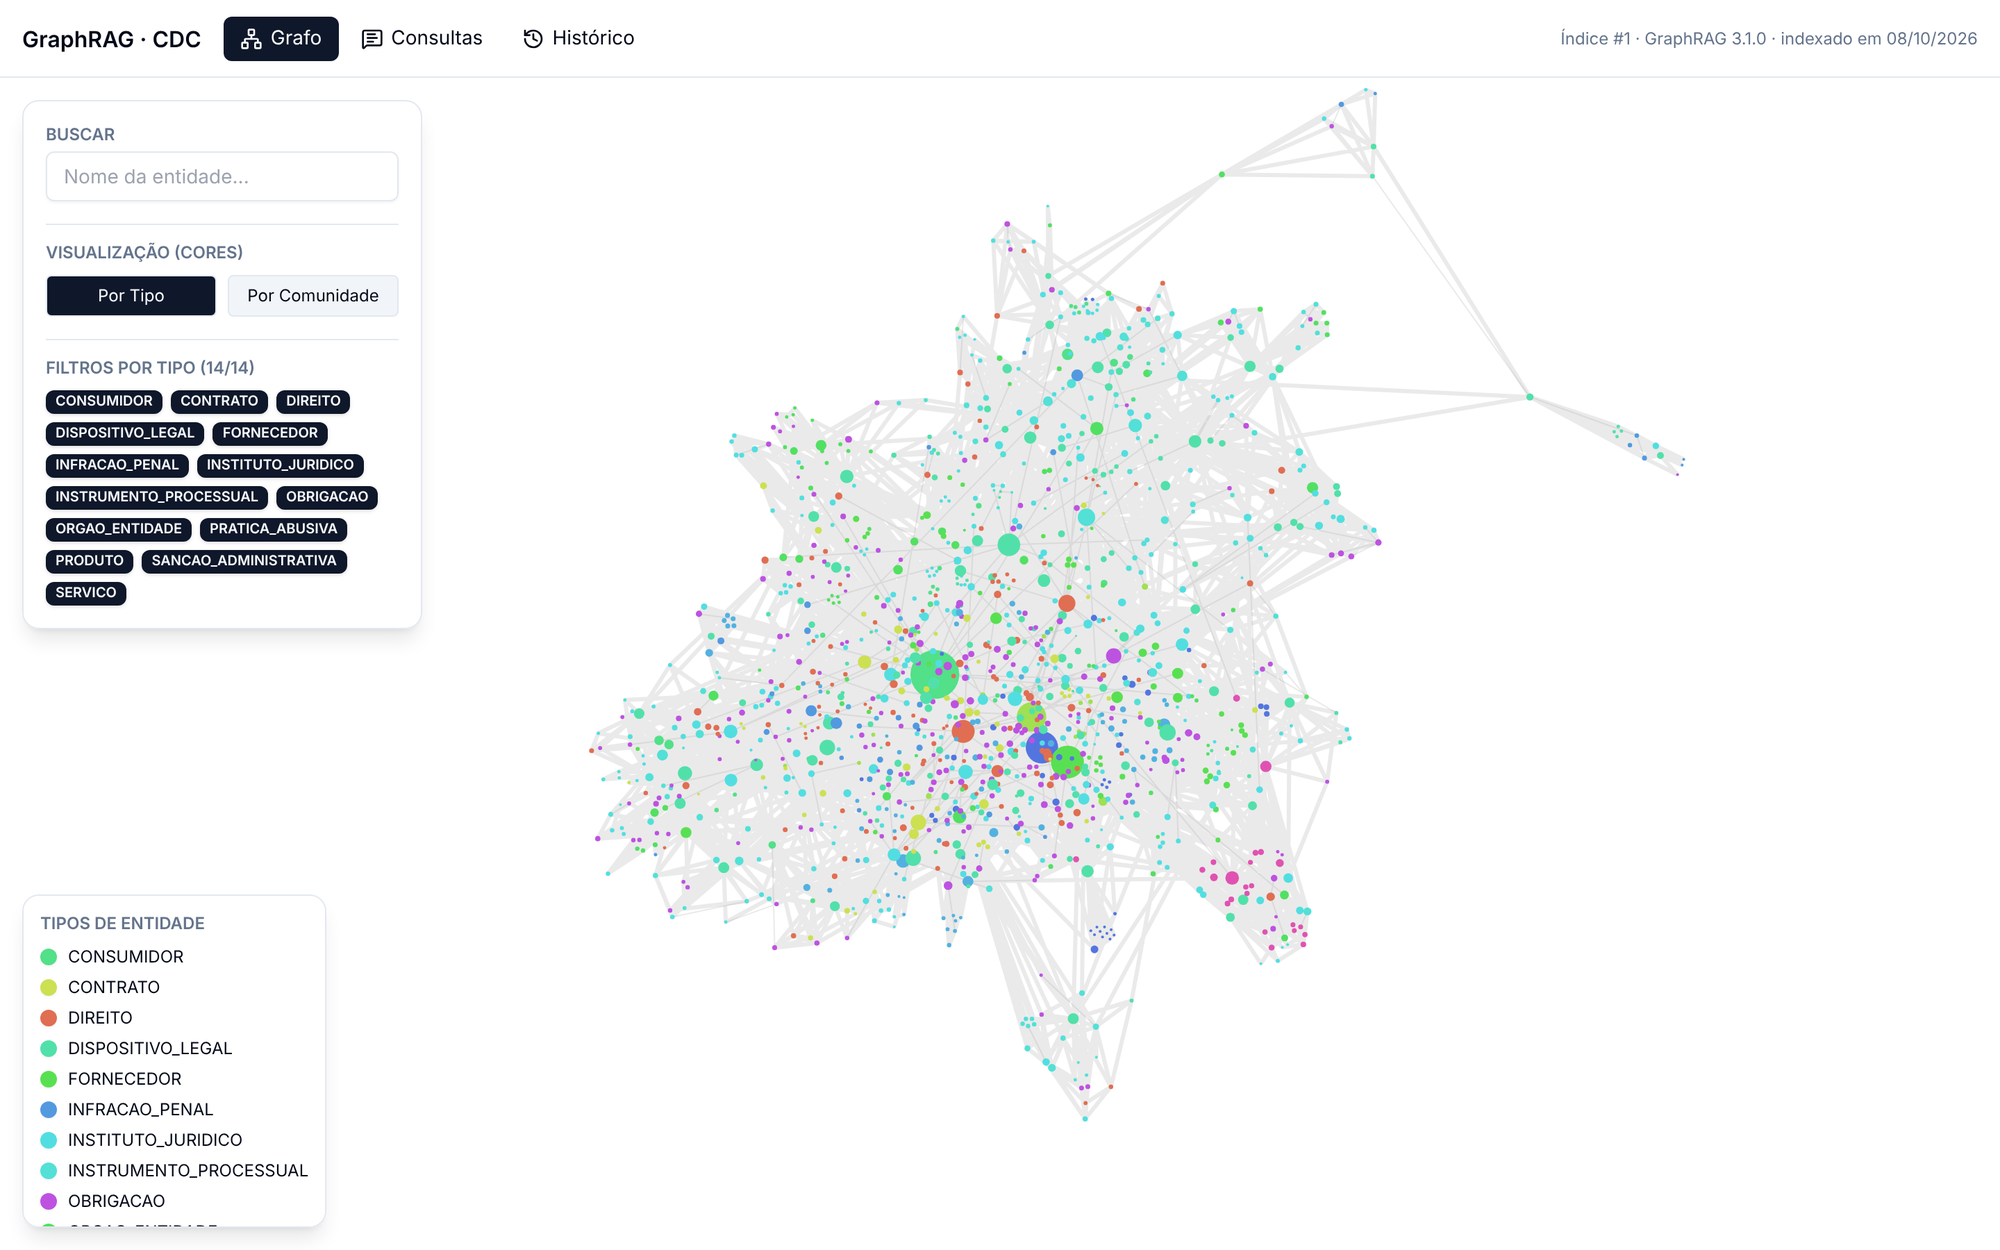
\includegraphics[width=\textwidth]{figuras/fig-app-grafo.png}
\caption{Grafo de conhecimento do CDC na aplicação web, com as entidades coloridas por tipo.}
\label{fig-grafo-completo}
\end{figure}

%%% Início de seção. %%%
\section{Custo da Indexação}
\label{sec-indexacao-custo}

A Tabela~\ref{tab-tokens-indexacao} apresenta o consumo de \textit{tokens} registrado pelo GraphRAG durante a indexação. O modelo principal fez 630 chamadas: 260 de extração (duas por unidade de texto, devido à rodada adicional) e as demais de geração dos 369 relatórios de comunidade. O modelo barato fez 406 chamadas de resumo de descrições.

\begin{table}[htb]
\centering
\caption{Consumo de \textit{tokens} da indexação.}
\label{tab-tokens-indexacao}
\footnotesize
\begin{tabular}{L{4.6cm} r r r}
\toprule
\textbf{Modelo} & \textbf{Chamadas} & \textbf{\textit{Tokens} de entrada} & \textbf{\textit{Tokens} de saída} \\
\midrule
\code{gpt-6.1-sol} & 630 & 4.303.693 & 1.471.243 \\
\code{gpt-6-luna} & 406 & 188.741 & 157.098 \\
\code{text-embedding-3-large} & 220 & 1.032.518 & -- \\
\bottomrule
\end{tabular}
\end{table}

O custo estimado pelos preços de tabela dos modelos ficou entre 16 e 24 dólares, enquanto a estimativa feita antes da indexação, a partir do tamanho do corpus, era de 3 a 6 dólares. A diferença veio principalmente dos \textit{tokens} de saída, os mais caros: a extração foi muito mais detalhada do que o previsto, com mais de 6.800 relações para um corpus de 130 artigos, e cada relação é acompanhada de uma descrição. Além disso, o \textit{prompt} de extração, com cerca de 11,7 mil \textit{tokens}, é enviado em todas as chamadas de extração, e os \textit{tokens} de raciocínio dos modelos utilizados são cobrados mas não aparecem nas contagens. A lição é que o custo do GraphRAG é dominado pela extração do grafo e pelos \textit{tokens} gerados, e que estimativas baseadas apenas no tamanho do corpus o subestimam.

%%% Início de seção. %%%
\section{Publicação e Reprodutibilidade}
\label{sec-indexacao-release}

Para que o índice possa ser reutilizado sem nova indexação, e para que a avaliação seja feita sobre um índice identificado e imutável, o resultado foi publicado como versão (\textit{release}) do repositório no GitHub, com a marcação \code{v0.1.0}, seguindo o versionamento semântico. O pacote contém as pastas de saída, cache e registros da indexação e cópias da configuração, dos \textit{prompts} e do corpus, nos caminhos originais, acompanhado de uma soma de verificação SHA-256, de um manifesto (versão do código, modelos, estatísticas do índice, consumo de \textit{tokens} e \textit{hashes} da configuração e dos \textit{prompts}) e de notas da versão com instruções de restauração. Nenhuma chave de API é incluída, o que foi verificado por busca de padrões de chave no pacote. A marcação \code{v1.0.0} foi reservada para o índice que será usado na avaliação final.

Como o cache das respostas dos modelos faz parte do pacote, quem restaurar a versão pode reexecutar a indexação com a mesma configuração praticamente sem custo, e verificar que o resultado é o mesmo. A versão do GraphRAG foi fixada em 3.1.0 em todos os ambientes, já que tanto o formato dos dados quanto o comportamento das consultas podem mudar entre versões.
